\documentclass[../main.tex]{subfile}
\graphicspath{{\subfix{../images}}}
\begin{document}

\subsection{可视化习得特征}\label{sec:pool5_vis}

第一层过滤器可以直接可视化,而且很容易理解\cite{alexnet}。它们能捕捉到定向的边缘和对手的颜色。理解后续层则更具挑战性。Zeiler和Fergus在\cite{adaptive}中提出了一种视觉上有吸引力的去卷积方法。我们提出了一个简单的(和互补的)非参数方法,直接显示网络学到了什么。

我们的想法是在网络中挑出一个特定的单元(特征),并将其作为一个物体检测器来使用。也就是说,我们计算出该单元在一大组被搁置的区域候选(大约1000万)上的激活,将这些建议从最高激活到最低激活进行排序,进行非最大抑制,然后显示出得分最高的区域。我们的方法让所选的单元 "为自己说话",准确地显示它在哪些输入上开火。我们避免平均化,以便看到不同的视觉模式,并深入了解该单元计算的不变性。

我们将pool5层的单元可视化,它是网络第五层也是最后一层卷积层的最大池化输出。pool5的特征图是$6\times 6\times 256 = 9216$维的。忽略边界效应,每个pool5单元在原始$227\times 227$像素的输入中具有$195\times 195$像素的感受野。一个中央的pool5单元有着几乎全局的视野,而靠近边缘的单元有较小的、被剪切的视野。

\begin{figure}[htb]
    \centering
    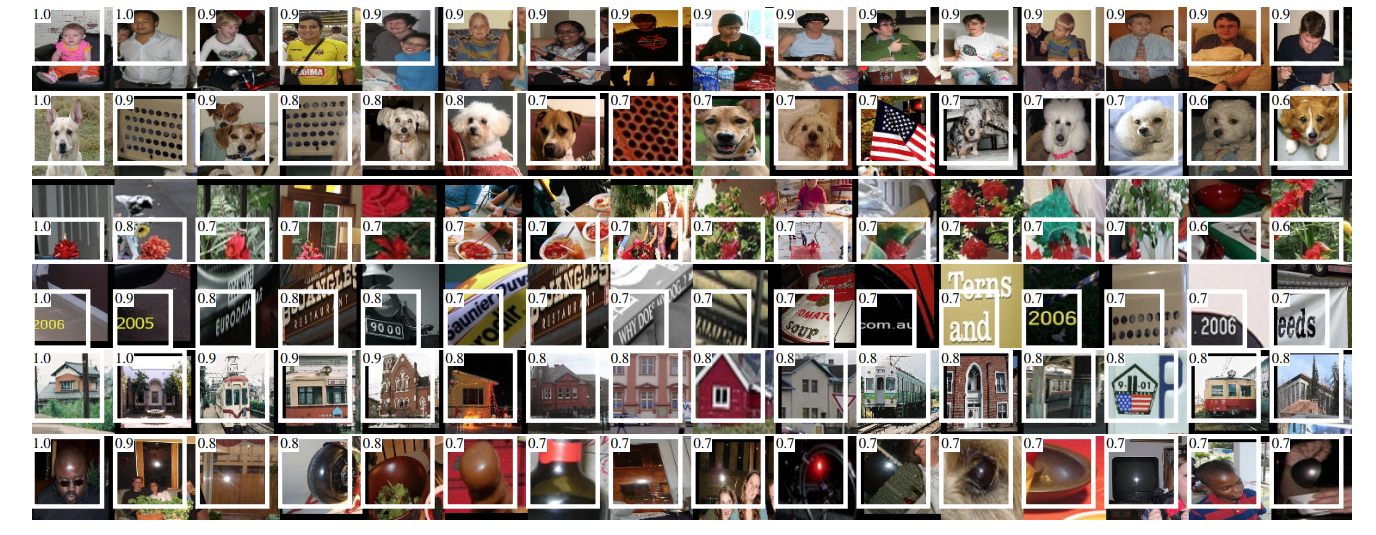
\includegraphics[width=\textwidth]{fig4.png}
    \caption{\textbf{六个pool5单元的顶部区域。}感受视野和激活值以白色绘制。一些单元与概念相一致,如人(第1行)或文本(4)。其他单元捕捉纹理和材料属性,如点阵(2)和镜面反射(6)。}
    \label{fig:fig4}
\end{figure}

图\ref{fig:fig4}中的每一行都显示了我们在VOC 2007 trainval上微调的CNN的pool5单元的前16个激活。在256个功能独特的单元中,有6个是做了可视化的(附录D包括更多)。选择这些单元是为了显示网络学习的代表性样本。在第二行,我们看到一个单元在狗脸和点阵上发射。第三行对应的单元是一个红色的圆球检测器。还有一些检测器用于检测人脸和更抽象的图案,如文字和带窗口的三角形结构。该网络似乎在学习一种表征,将少量的类调整特征与形状、纹理、颜色和材料属性的分布式表征结合在一起。随后的全连接层fc6有能力对这些丰富特征的大量组合进行建模。

\subsection{消融实验} \label{sec:ablation}

\paragraph{在无微调设置下的逐层性能。}

为了了解哪些层对检测性能至关重要,我们分析了CNN最后三层中每一层在VOC 2007数据集上的结果。第\ref{sec:pool5_vis}节中简要介绍了pool5。下面总结了最后两层的情况。

fc6层与pool5完全连接。为了计算特征,它用一个$4096\times 9216$的权重矩阵乘以pool5的特征图(重塑为9216维的向量),然后加上一个偏置向量。这个中间向量的每一个分量都要经过半波整流($x = \max(0; x)$)。

fc7层是网络的最后一层。它是通过将fc6计算出的特征乘以$4096\times 4096$的权重矩阵来实现的,同样地,加入一个偏置矢量并应用半波整流。

我们首先看一下没有在PASCAL上进行微调的CNN的结果,即所有的CNN参数都只在ILSVRC 2012上进行了预训练。逐层分析性能(表2第1-3行),发现fc7的特征比fc6的特征泛化性能差。这意味着29\%,即大约1680万个CNN的参数可以被移除而不降低mAP。更令人惊讶的是,尽管pool5的特征只用了CNN的6\%的参数计算,但去除fc7和fc6都会产生相当好的结果。CNN的大部分表征能力来自其卷积层,而不是来自更大的密集连接层。这一发现表明,只用CNN的卷积层就能计算出任意大小图像的密集特征图,即HOG的意义。这种表示方法将使人们能够在pool5特征的基础上进行滑动窗口检测器的实验,包括DPM。

\paragraph{在微调设置下的逐层性能。}

我们现在看看我们的CNN在VOC 2007 trainval上微调了参数后的结果。改进是惊人的(表2第4-6行):微调使mAP增加了8.0个百分点,达到54.2\%。微调对fc6和fc7的提升比对pool5的提升要大得多,这表明从ImageNet学到的pool5特征是通用的,大部分的改进是通过在它们上面学习特定领域的非线性分类器获得的。

\paragraph{与近期特征学习方法的比较。}

相对来说,在PASCAL VOC检测上尝试的特征学习方法很少。我们看一下最近两种建立在可变形部件模型上的方法。作为参考,我们也包括基于HOG的标准DPM\cite{dpm}的结果。

第一种DPM特征学习方法,DPM ST [28],用 "草图标记 "概率直方图来增强HOG特征。直观地说,草图标记是通过图像斑块中心的轮廓线的紧密分布。草图标记概率是由一个随机森林在每个像素上计算出来的,该随机森林被训练成将35×35像素的斑块分类为150个草图标记或背景之一。

第二种方法,DPM HSC[31],用稀疏编码直方图(HSC)取代了HOG。为了计算HSC,使用100个$7\times 7$像素(灰度)原子的学习字典来解决每个像素的稀疏代码激活问题。得到的激活以三种方式(全波和半波)进行整顿,空间汇集,单位$\ell_2$归一化,然后进行功率变换($x \gets \text{sign}(x)\vert x \vert^\alpha $)。

所有的R-CNN变体都强烈地超越了三个DPM基线(表2第8-10行),包括使用特征学习的两个变体。与只使用HOG特征的DPM的最新版本相比,我们的mAP高出20多个百分点:54.2\%对33.7\%——61\%的相对改进。HOG和草图标记的组合比单独的HOG产生了2.5个mAP点,而HSC比HOG提高了4个mAP点(当与他们的私有DPM基线进行内部比较时--两者都使用了DPM的非公开实现,性能低于开源版本[20])。这些方法的mAPs分别为29.1\%和34.3\%。

\subsection{网络结构}

本文中的大多数结果都使用了Krizhevsky等人\cite{alexnet}的网络架构。然而,我们发现,架构的选择对R-CNN的检测性能有很大的影响。在表3中,我们展示了使用Simonyan和Zisserman\cite{vgg}最近提出的16层深度网络对VOC 2007测试的结果。这个网络是最近ILSVRC 2014分类挑战中表现最好的网络之一。该网络有一个同质的结构,由13层3×3卷积核组成,中间穿插着5个最大池化层,顶部是三个全连接层。我们把这个网络称为 "O-Net",即OxfordNet,把基线称为 "T-Net",即TorontoNet。

为了在R-CNN中使用O-Net,我们从Caffe Model Zoo1中下载了公开可用的\lstinline{VGG_ILSVRC_16_layers}模型的预训练网络权重,然后使用与T-Net相同的协议对网络进行微调。唯一的区别是使用较小的迷你批(24个例子),以适应GPU内存的需要。表3中的结果显示,使用O-Net的R-CNN大大优于使用T-Net的R-CNN,将mAP从58.5\%提高到66.0\%。然而,在计算时间方面有一个相当大的缺点,O-Net的前向传递大约比T-Net长7倍。

\subsection{检测误差分析}

我们应用了Hoiem等人\cite{diagnosing}的优秀检测分析工具,以揭示我们方法的错误模式,了解微调如何改变它们,并查看我们的错误类型与DPM的比较。对分析工具的全面总结超出了本文的范围,我们鼓励读者查阅\cite{diagnosing}以了解一些更精细的细节(如 "规范化AP")。由于分析最好是在相关图表的背景下进行,我们在图\ref{fig:fig5}和图\ref{fig:fig6}的字幕中进行了讨论。

\begin{figure}[H]
    \centering
    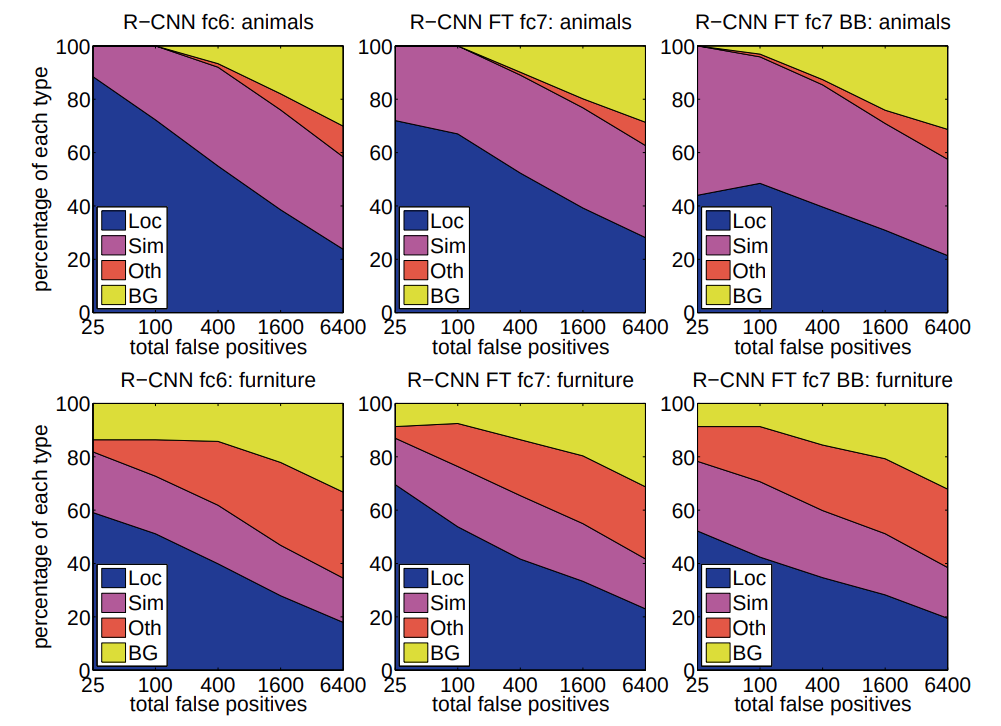
\includegraphics[width=\textwidth]{fig5.png}
    \caption{\textbf{排名靠前的误报(fasle positive, FP)类型的分布。}每幅图显示了随着分数递减产生更多误报,误报类型的演变分布。每个FP被分为4种类型中的一种:Loc-差的定位(与正确类别的IoU重叠在0.1和0.5之间的检测,或重复);Sim-与相似类别的混淆;Oth-与不相似物体类别的混淆;BG-在背景上发射的误报。与DPM相比(见\cite{dpm}),我们的错误中明显有更多是由于定位不准确造成的,而不是与背景或其他物体类别的混淆,这表明CNN的特征比HOG更具有分辨力。松散的定位可能是由于我们使用了自下而上的区域候选和从预先训练整个图像分类的CNN中学到的位置不变性。第三栏显示了我们简单的边界盒回归方法如何解决了许多定位错误。}
    \label{fig:fig5}
\end{figure}

\subsection{边界框回归}

基于误差分析,我们实现了一个简单的方法来减少定位误差。受DPM\cite{dpm}中采用的边界盒回归的启发,对于一个选择性搜索区域,给定pool5的特征,我们训练了一个线性回归模型,以预测一个新的检测窗口。完整的细节在附录C中给出。表1、表2和图\ref{fig:fig5}中的结果显示,这种简单的方法修复了大量的错误定位的检测,使mAP提高了3到4个点。

\begin{figure}[H]
    \centering
    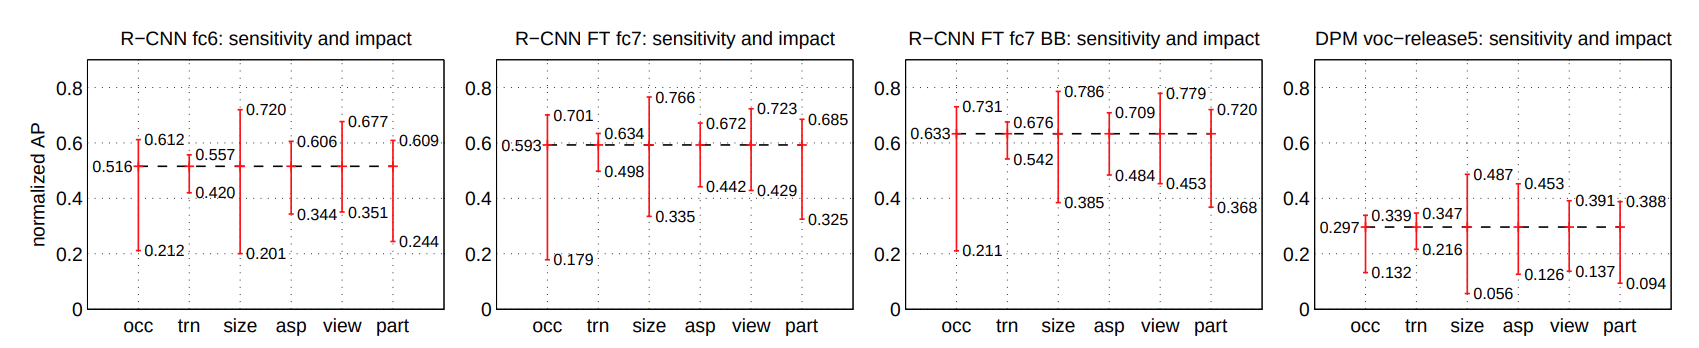
\includegraphics[width=\textwidth]{fig6.png}
    \caption{\textbf{对物体特征的敏感性。}每张图都显示了在六个不同的物体特征(遮挡、截断、边界框面积、长宽比、视角、部分可见)中,最高和最低性能子集的平均(所有类别)归一化AP(见\cite{dpm})。我们展示了我们的方法(R-CNN)在有微调(FT)和无微调(BB)以及DPM voc-release5的情况下的图表。总的来说,微调并没有降低灵敏度(最大和最小之间的差异),但对于几乎所有的特征来说,微调确实大大改善了最高和最低性能子集。这表明,微调不仅仅是简单地改善了长宽比和边界盒面积的最低性能子集,正如人们根据我们如何扭曲网络输入所猜想的那样。相反,微调提高了所有特征的鲁棒性,包括遮挡、截断、视角和部件的可见性。}
    \label{fig:fig6}
\end{figure}



\end{document}

